\documentclass{article}

% if you need to pass options to natbib, use, e.g.:
% \PassOptionsToPackage{numbers, compress}{natbib}
% before loading nips_2016
%
% to avoid loading the natbib package, add option nonatbib:
% \usepackage[nonatbib]{nips_2016}

\usepackage{nips_2016}

% to compile a camera-ready version, add the [final] option, e.g.:
% \usepackage[final]{nips_2016}

\usepackage[utf8]{inputenc} % allow utf-8 input
\usepackage[T1]{fontenc}    % use 8-bit T1 fonts
\usepackage{hyperref}       % hyperlinks
\usepackage{url}            % simple URL typesetting
\usepackage{booktabs}       % professional-quality tables
\usepackage{amsfonts}       % blackboard math symbols
\usepackage{nicefrac}       % compact symbols for 1/2, etc.
\usepackage{microtype}      % microtypography
%\usepackage[english]{babel}
%\usepackage{cite}
%\usepackage{verbatim}
\usepackage{amsmath}
\usepackage{amssymb,amsbsy,epsfig,float}
\usepackage{graphicx,wrapfig,lipsum}
%\usepackage{graphicx}
%\usepackage{multirow}
%\usepackage{algorithmicx}
%\usepackage[ruled]{algorithm}
%\usepackage{algpseudocode}


\newtheorem{thm}{Theorem}
\newtheorem{lemma}{Lemma}
\newtheorem{proposition}{Proposition}
\newtheorem{corol}{Corollary}
\newtheorem{example}{Example}
\newtheorem{remark}{Remark}
\newtheorem{definition}{Definition}
\newtheorem{assumption}{Assumption}
%\newcommand{\one}[1]{\boldsymbol{1}_{#1}}
%\newcommand{\Prob}[1]{\Pr\{#1\}}
%\newcommand{\EE}[1]{\mathbb{E}[#1]}
%\DeclareMathOperator{\sgn}{sgn}

\title{Label Free Resource-Constrained Learning}

% The \author macro works with any number of authors. There are two
% commands used to separate the names and addresses of multiple
% authors: \And and \AND.
%
% Using \And between authors leaves it to LaTeX to determine where to
% break the lines. Using \AND forces a line break at that point. So,
% if LaTeX puts 3 of 4 authors names on the first line, and the last
% on the second line, try using \AND instead of \And before the third
% author name.

\author{
	David S.~Hippocampus\thanks{Use footnote for providing further
		information about author (webpage, alternative
		address)---\emph{not} for acknowledging funding agencies.} \\
	Department of Computer Science\\
	Cranberry-Lemon University\\
	Pittsburgh, PA 15213 \\
	\texttt{hippo@cs.cranberry-lemon.edu} \\
	%% examples of more authors
	%% \And
	%% Coauthor \\
	%% Affiliation \\
	%% Address \\
	%% \texttt{email} \\
	%% \AND
	%% Coauthor \\
	%% Affiliation \\
	%% Address \\
	%% \texttt{email} \\
	%% \And
	%% Coauthor \\
	%% Affiliation \\
	%% Address \\
	%% \texttt{email} \\
	%% \And
	%% Coauthor \\
	%% Affiliation \\
	%% Address \\
	%% \texttt{email} \\
}

\begin{document}
	% \nipsfinalcopy is no longer used
	
	\maketitle
	
	\begin{abstract}
		Abstract goes here
	\end{abstract}

\section{Introduction}
In many classification systems  such as medical diagnosis  and  homeland  security,  sequential decisions  are  often  warranted.   For each  instance,  an initial diagnostic test  is conducted and based on its results further tests maybe conducted. Tests have varying  costs for  acquisition,  and  these  costs  account  for delay,  throughput  or  monetary  value \footnote{As described in \cite{Trapeznikov} security systems utilize a suite of sensors/tests such as X-rays, millimeter wave imagers (expen-
sive \& low-throughput), magnetometers, video, IR imagers human search.  Security systems  must  maintain  a  throughput  constraint  in  order to  keep  pace  with  arriving  traffic.   In  clinical  diagnosis, doctors  in the context of breast cancer diagnosis utilize tests such as genetic markers, imaging (CT, ultrasound, elastography) and biopsy. Sensors providing imagery are scored by humans. The different sensing  modalities  have  diverse  costs,  in  terms  of  health risks (radiation exposure) and monetary expense.}. 

Our goal in this paper is to identify the most accurate and cost-effective tests/sensors to acquire given an instance (and its context). We assume that the sensors/tests are organized into a diagnostic tree architecture with the least informative and inexpensive sensors at the higher levels of the tree. Nodes of the tree correspond to a test that outputs a prediction of the underlying state of the instance (disease or disease-free, threat or no-threat etc.). Based on information obtained from tests along the unique path from root to the node, a decision is made as to whether or not a subsequent test may be required. This perspective is reasonable in medical diagnostic and surveillance systems where cascades/trees of sensing tests are pre-defined. Our objective is to learn a decision rule that  utilizes  inexpensive tests for majority of instances and requests the expensive (and more informative) only for the few difficult ones. Such a strategy maintains classifier accuracy while reducing the average acquisition cost per decision. 

We assume that the classifiers (or predictors) corresponding to each node are pre-defined and produce labeled outputs. This is often the case in diagnostic systems where a report is produced by a human being or a automated classification mechanism based on sensor measurements. Thus our task in this paper is to learn a decision rule to identify the collection of tests required for an instance. 

Our problem can be framed as a version of a multi-armed bandit problem. Each arm of the bandit corresponds to a unique path from root to a node where the observation is a vector of outputs from tests acquired along that path. Nevertheless, unlike a conventional bandit problem, where a reward is observed corresponding to each action, 


1. sequential resource constrained prediction arises in medical diagnosis and security applications.
2. many sensor systems have pre-existing classifiers or utilize human classifiers. The output of these systems come in the form of predictions.
3.  We assume that informative sensors are costly, cause large delays but generally give better accuracy. 
4. we consider the setting where we do not get to see either a noiseless or a noisy version of the true ground-truth label. while the general setting resembles multi-armed bandit problem it is different in the sense that we do not have access to the reward. We can only observe the predictions. 
5. We are given a network tree of sensors where the root is assumed to be least expensive and least informative sensor. We assume that the sensors are organized into a hierarchy of expensive and informative sensors. The goal is to identify for each instance which sensor(s) to use based on previous sensor predictions.


%The quality of sensors used in a decision system influences the accuracy of  the measurements or the predictions. Typically, a less accurate sensor is cheap and produces predictions faster. A more accurate sensor is costly and takes more time to output predictions. In practice, the budget/time constraints do not allow costly/slow sensors to be used all the time and one has to use the sensor that is the most `cost effective'. One natural way is to use a sensor for which sum of prediction error rate and cost is the lowest. However,  values of the errors rate may not be known a priori and the best cost effective sensor cannot be determined. Further, the true labels required to estimate the error rate may also be not available or prohibitively expensive to know. In this paper we study the problem of learning the most cost effective sensor when the true labels are not known, and the goal is to efficiently learn the most cost effective sensor. 



{\it In summary: \\
	1. there is a test-time acquisition problem. This is not us. Because we do not have annotated training data. \\
	2. This is not an online version of test-time acquisition problem. Because we do not get ground truth labels for the predictions we make.\\
	3. We are in a situation where we have a network of sensors and their predictions if and when we probe those sensors. Our situation is such that we observe the predictions of the sensors in the directed neighborhood of the probed sensor.\\
	4. Thus we do not directly observe the label and the situation resembles a online/bandit setting but without observing either a noisy or noiseless version of the reward.\\
	5. This situation arises in Homeland security as well as in medical diagnosis.}

This problem arises in many applications including homeland security, communication networks and medical diagnosis. For example, in the homeland security problem, where bags need to be screened for potential threats, either a cheap Infra-red (IR) imager or a more expensive and time consuming active millimeter wave (AMMW) scanner can be used. In medical diagnosis, practitioners can use non-invasive blood test, CT scan to determine a medical condition or go for a more invasive surgical procedures. In wireless communications, network designer can use error correcting codes of different block lengths to overcome channel noise. A code with higher block length (more redundancy)  improve the tolerance against noise but reduces transmission rate. 
     
Several papers including \cite{AISTATS13_SupervisedSequentialLearning_TrapezSaligram},\cite{ML13_MultistageClassifier_TrapezSaligramaCastanon}\cite{ICML13_CostSensitiveTreeClassification_XuKusnerChenWeinberger} have considered the problem of learning the best cost effective predictor/classifier using supervised learning methods. The general approach in these methods is to learn a decision function by minimizing an empirical risk objective over a training set. The objective functions in these methods are inherently non-convex and the authors resort to convex relaxations and experimental validations without any theoretical guarantees. However, in many applications gathering training samples may be infeasible, and moreover the labels may not be available at all. We consider an online version of this problem where the samples arrive sequentially and a learner has to decide which sensors to apply for prediction. For each sample, the learner only observes sensor predictions and true label is not revealed. 

In this work we focus on sequential predication of binary labels.  Similar to \cite{ML13_MultistageClassifier_TrapezSaligramaCastanon}, we consider that the order in which sensors are applied is fixed. Typically, the cheapest sensor, or the one with highest error rate, is used first, followed by next cheap sensor with smaller error rate and so on. The sensors thus constitute stages of a cascade, where prediction error rates decrease along the depth, while the costs increase. For each new sample, the learner applies the sensors sequentially and can stop at any stage in the cascade. The goal is to stop at a stage where expected loss is the smallest. Loss at depth $k$ is defined as total cost incurred for acquiring sensor predictions plus a penalty which is $1$ if the prediction of $k^{th}$ sensor is correct, otherwise it is zero. If the learner stops at a depth $k$, he obtains the predictions of all the first $k$ senors as feedback, but which of them are correct is unknown. We refer to this setup as the Sensor Acquisitions Problem (SAP). 

The feedback in SAP do not reveal information about the losses, hence the learner cannot identify the best stage for any sample. 
We thus focus on scenarios where feedback satisfies some stochastic ordering. Specifically, we assume that if a sensor in the cascade predicts a label correctly, any subsequent sensor also predict it correctly. We refer to this assumption as {\em dominance condition}. When it holds, the learner can partially infer losses of the stages, which, as discussed later, is sufficient to learn the best stage for a given sample. We further demonstrate that under any weaker condition the learner cannot identify the best stage. Dominance conditions holds in many scenarios includes the examples discussed at the beginning. In the wireless communication example, if an error correcting code (ex. Reed-Solomon, LDPC \cite{Book_InferenceLearning_MacKay} recovers information in a channel with certain noise level, then with more redundancy blocks in the error correction code we can certainly recover the information on the channel (though at a lower transmission rate).     

Our first main contribution is to show that if the dominance condition holds the SAP problem can be reduced to 
a stochastic multi-armed bandit with side observations,
where bandit arms are identified with the stage of cascade,
the payoff of an arm is given by loss from the corresponding stage, and side observation structure is defined by the feedback graph induced by the cascade. In particular, we show that the SAPregret
of any meta-strategy is equal to its bandit-regret
when the procedure is used to play in the corresponding
bandit problem. As a consequence, we conclude that existing efficient
bandit algorithms, as well as their bounds on bandit-regret,
can be directly applied to achieve new results
for SAP. Although the underlying
reduction is straightforward, it gives ready policies with performance guarantees for SAP and their fundamental limitations .


Related Work: \cite{AISTATS13_SupervisedSequentialLearning_TrapezSaligram}\cite{ICML14_PredictionWithLimitedAdvice_LattimoreCrammerCzepes}

Structure of paper

\section{Sensor Acquisition Problem}
\label{sec:Setup}
%The sensors are differentiated in terms of their prediction efficiency and cost. 
The learner has access to $K\geq 2$ sensors that are ordered in terms of their prediction efficiency. Specifically, we consider that the sensors form a cascade (order in which the sensors are selected is predetermined) and in each round the learner can sequentially select a subset of sensors in the cascade and stop at any depth.  

Let $\{Z_t, Y_t\}_{{t>0}}$ denote a sequence generated according to an unknown distribution. $Z_t \in\mathcal{C} \subset  \mathcal{R}^d$, where $\mathcal{C}$ is a compact set, denotes a feature vector/context at time $t$ and $Y_t \in \{0,1\}$ its binary label. We denote output/prediction of the $i^{th}$ sensor as $\hat{Y}^i_t$ when its input is $Z_t$. The set of actions available to the learner is $\mathcal{A}=\{1,\ldots, K\}$, where  the action $k \in \mathcal{A}$ indicates acquiring predictions from sensors $1,\ldots, k$ and classifying using the prediction $\hat{Y}^k_t$. 


\begin{wrapfigure}{r}{5cm}
	\vspace{-.5cm}
	\centering
	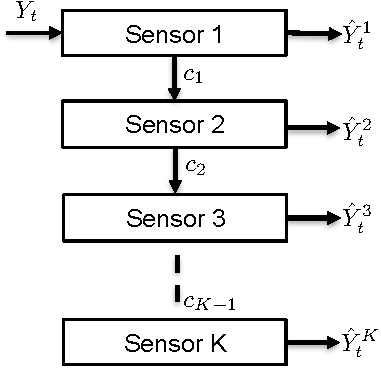
\includegraphics[scale=.6]{SensorCascade.pdf}
	\caption{Cascade of sensors}\label{wrap-fig:1}
    \vspace{-.5cm}
\end{wrapfigure} 

The prediction error rate of the $i^{th}$ sensor is denoted as $\gamma_i:=\Pr\{Y_t\neq \hat{Y}^k_t\}$. In this section we assume that the error rate does not depend on the  context and postpone the treatment with contextual information to Section \ref{sec:Contextual}. Further, the sensors are arranged such that the prediction error rate improves with depth in the cascade, i.e., $\gamma_{k-1}\geq \gamma_k$ for all $k>2$. However, the learner incurs an extra cost of $c_k\geq 0$ to acquire output of sensor $k$ after acquiring output of sensor $k-1$. The sensor cascade is depicted in the adjacent figure.

Let $H_t(k)$ denote the feedback observed in round $t$ from action $k$. Since we observe predictions of all the first $k$ senors by playing action $k$, we get   $H_t(k)=\{\hat{Y}^1_t,\ldots,\hat{Y}^k_t\}$.
The loss incurred in each round is defined in terms of the prediction error and the total cost involved. When the learner selects action $k$, loss is the prediction error of sensor $k$ plus sum of the costs incurred along the path ($c_1,\ldots,c_k$). Let $L_t: \mathcal{A}\rightarrow \mathcal{R}_+$ denote the loss function in round $t$. Then,
\begin{equation}
L_t(k)=\mathbf{1}_{\{\hat{Y}^k_t\neq Y_t\}}+\sum_{j=1}^k c_j.
\end{equation} 
We refer to the above setup as Sensor Acquisition Problem (SAP) and denote it as $\psi=(K,\mathcal{A}, (\gamma_i,c_{i-1})_{i\in [K]})$\footnote{Note that $k\in \mathcal{A}$ implies that action $k$ selects all sensors ${1, 2, \cdots, k}$, not just sensor $k$. We set $c_0=0$}. A policy $\pi^\psi=(\pi^\psi_1, \pi^\psi_2, \cdots)$ on $\psi$, where  $\pi^\psi_t : \mathcal{H}_{t-1}\rightarrow
\mathcal{A}$, gives action selected in each round using history $\mathcal{H}_{t-1}$ that consists of all actions and corresponding feedback observed before $t$. Let $\Pi^\psi$ denote set of policies on $\psi$. For any $\pi \in \Pi^\psi$, we compare its performance with respect to the optimal policy (single best action in hindsight) and define its expected regret as follows
\begin{equation}
R^\psi_T(\pi)= \mathbb{E}\left[\sum_{t=1}^T L_t(a_t)\right]-\min_{k\in A}\mathbb{E}\left[\sum_{t=1}^T L_t(k)\right],
\end{equation}
where $a_t$ denotes the policy selected by $\pi_t$ in round $t$.
The goal of the learner is to learn a policy that minimizes the expected total loss, or, equivalently, to minimize the expected regret, i.e.,
\begin{equation}
\pi^*= \arg \min_{\pi \in \Pi^\psi } R^\psi_T(\pi).
\end{equation}

\noindent
{\bf Optimal action in hindsight: } For any $t$, we have 
\begin{equation}
\label{eqn:OptimalAction}
\mathbb{E}[L_t(k)]=\Pr\{Y_t\neq \hat{Y}^k_t\}+\sum_{j=1}^kc_j=\gamma_k +\sum_{j=1}^kc_j.
\end{equation}
Let $k^*=\arg\min_{k\in \mathcal{A}} \gamma_k + \sum_{i< k}c_i$. Then the optimal policy is to play action $k^*$ in each round. If an action $i$ is played in any round then it adds   $\Delta_k:=\gamma_k + \sum_{i<k}c_i -( \gamma_{k^*} + \sum_{i<k^*}c_i)$ to the expected regret. Let $I_t$ denote the action selected in round $t$ and $N^\psi_k(s)$ denote the number of times action $k$ is selected till time $s$, i.e., $N^\psi_k(s)=\sum_{t=1}^s \boldsymbol{1}_{\{I_t=k\}}$. Then the expected regret can be expressed as
\begin{eqnarray}
\label{eqn:ExpRegretGap}
R^\psi_T(\pi)&=& \sum_{k \in \mathcal{A}}\mathbb{E}[N_k^\psi(T)]\Delta_k.
\end{eqnarray}\


\section{When is SAP Learnable?}
In the SA-Problem feedback $H_t(\cdot)$ does not reveal any information about the true label $Y_t$ in any round $t$. Hence the loss values are not known, and we are in a hopeless situation where linear regret is unavoidable. In this section we explore conditions that lead to policies that are Hannan consistent \cite{Hannan1957_HannanConsistency_Hannan}, i.e, a policy $\pi\in \Pi^\psi$ such that $R_T^\psi (\pi)/T \rightarrow 0$.

Let us consider $K=2$ sensors and start with a simple condition that if sensor $1$ predicts the label $1$ correctly, then sensor $2$ also predicts it correctly\footnote{Suppose we interpret label $1$ as 'threat', the condition implies that if sensor $1$ detects threat correctly, the better sensor $2$ also detects it. }, i.e.,
\begin{equation}
\label{eqn:PathDominace1} 
Y_t=1 \mbox{ and } \hat{Y}_t^1=1 \implies \hat{Y}^2_t=1. 
\end{equation}
To fix ideas, we enumerate all the $8$ possible tuples $(Y, \hat{Y}^1, \hat{Y}^2)$ as shown in Table \ref{tab:SensorOutcomes}, and write probability of the $i$th tuple $i=1,2,\cdots 8$ as $p_{i-1}$.  From Table \ref{tab:SensorOutcomes}, we have  $\gamma_1=p_2+p_3+p_4+p_5$ and $\gamma_2=p_1+p_3+p_4+p_6$, thus
\begin{equation}
	\gamma_1-\gamma_2 = p_2+p_5-p_1-p_6.
\end{equation}

\begin{minipage}{0.5\textwidth}
	\vspace{.5cm}
	\begin{tabular}[c]{ c|c|c|c } 
		\label{tab:SensorOutcomes}
	%			\caption{Possible binary tuples}
		$Y$ & $\hat{Y}_t^1$ & $\hat{Y}_t^2$ & $\Pr(Y, \hat{Y}^1, \hat{Y}^2)$ \\ \hline 
		$0$ & $0$ & $0$ & $p_0$ \\  \hline
		$0$ & $0$ & $1$ & $p_1$ \\  \hline
		$0$ & $1$ & $0$ & $p_2$ \\  \hline
		$0$ & $1$ & $1$ & $p_3$ \\  \hline
		$1$ & $0$ & $0$ & $p_4$ \\  \hline
		$1$ & $0$ & $1$ & $p_5$ \\  \hline
		$1$ & $1$ & $0$ & $p_6$ \\  \hline
		$1$ & $1$ & $1$ & $p_7$ \\  \hline
		
	\end{tabular}
		\vspace{.5cm}
\end{minipage}\hspace{-1.5cm}
\begin{minipage}[c]{0.6\textwidth}
		\vspace{.5cm}
		\centering
	\hspace{-5cm}		
\begin{equation}
\label{eqn:Marginals}
\Pr(\hat{Y}^1, \hat{Y}^2)=
\begin{cases}
p_1 + p_5 \mbox{  if } (\hat{Y}^1, \hat{Y}^2)=(0,1)\\
p_2 + p_6 \mbox{  if } (\hat{Y}^1, \hat{Y}^2)=(1,0)\\
p_0 + p_4 \mbox{  if } (\hat{Y}^1, \hat{Y}^2)=(0,0)\\
p_3 + p_7 \mbox{  if } (\hat{Y}^1, \hat{Y}^2)=(1,1)
\end{cases}
\end{equation}
	\vspace{.5cm}
\end{minipage}

\noindent
From (\ref{eqn:OptimalAction}), action $1$ is optimal if $\gamma_1 - \gamma_2 \leq c$, otherwise action $2$ is optimal. If a policy learns the difference $\gamma_1-\gamma_2$, it can play the optimal arm and it is Hannan consistent. Note that only sensor output $(\hat{Y}^1, \hat{Y}^2)$ are observed and not the true label $Y$. Hence only values of marginal probabilities $\Pr(\hat{Y}^1, \hat{Y}^2)$ as given in (\ref{eqn:Marginals}) can be used to learn the difference $\gamma_1-\gamma_2$. The following example demonstrate that just knowing the values of marginals is not enough to decide which action is optimal.

Set $c=0.35$ and consider the following two case: 1) $p_2=1/2, p_1=1/4-1/40, p_5=1/4+1/40$ and 2) $p_2=1/2, p_1=1/4-3/40,p_5=1/4+3/40$. From condition (\ref{eqn:PathDominace1}) we have $p_6=0$. Also, set $p_0=p_4=p_3=p_7=0$ in both the cases. We get $\gamma_1-\gamma_2=0.3$ in the first case, hence action $1$ is optimal. Where as $\gamma_1-\gamma_2=0.4$ in the second case, hence actions $2$ is optimal. However, for both the cases the marginals $\Pr(\hat{Y}^1, \hat{Y}^1)$ are the same for all pairs $(\hat{Y}^1, \hat{Y}^1)$. Since we only observer the pairs $(\hat{Y}^1, \hat{Y}^1)$, one cannot hope to distinguish the cases and linear regret is unavoidable. 

Next, assume that  if sensor $0$ predicts the label $0$ correctly, then sensor $2$ also predicts it correctly, i.e.,
\begin{equation}
\label{eqn:PathDominace2} 
Y_t=0 \mbox{ and } \hat{Y}_t^1=0 \implies \hat{Y}^2_t=0. 
\end{equation}
We can argue similar to the previous example that under this conditions one cannot expect better than linear regret. Now assume that both (\ref{eqn:PathDominace1}) and (\ref{eqn:PathDominace2}) hold. Then, $p_2=p_6=0$ and we get $\gamma_1-\gamma_2=p_5-p_1$. Since $p_5=\Pr(0,1)$ and $p_1=\Pr(1,0)$, we can learn their values by observing $(0,1)$ and $(1,0)$ patterns and thus hope for a Hannan consistent policy. In the following we assume that (\ref{eqn:PathDominace1}) and (\ref{eqn:PathDominace2}) hold and refer to it as dominance condition. For the case of $K>2$ sensors, it is given as follows: 

\begin{assumption}[Dominance Condition]
	If sensor $i$ predicts correctly, all the sensors in the subsequent stages of the cascade also predict correctly, i.e.,
	
	\begin{equation}
	\label{eqn:DominanceCondition}
	\hat{Y}_t^i=Y_t \rightarrow \hat{Y}_t^j \quad \forall j>i\geq 1
	\end{equation}
\end{assumption}
In the following we establish that under the dominance condition efficient algorithms for a SAP problem can be derived from algorithms on a suitable stochastic multi-armed bandit problem. We first recall the stochastic multi-armed bandit setting and the relevant results. 

%\section{Problem Setup}
%\label{sec:Setup}
%We consider the problem of efficient label prediction under partial monitoring. Let $\{Y_t\}_{{t>0}}$ denote sequence of labels generated according to an unknown distribution $\mathcal{D}$.  The learner can use a `cheap' sensor (device-1) or/and a `costly' sensor (device-2) to predict the labels. In round $t$, let $\hat{Y}^1_t$ and $\hat{Y}^2_t$ denote the predictions of device-1 and device-2 respectively. We assume that device-1 has lower performance than device-2 in the sense that prediction error rate of device-1, denoted as 
%$\gamma_1:=\Pr\{Y_t\neq \hat{Y}^1_t\}$, is larger than or equal to that of device-2, denoted as $\gamma_2:=\Pr\{Y_t\neq \hat{Y}^2_t\}$ ($\gamma_1>\gamma_2$). In each round $t$, the learner can take the following actions: 
%\begin{itemize}
%	\item Action-1: use device-1.
% \item Action-2: use both the devices. 
%\end{itemize}
%For ease of notion, we denote actions by their index, and write $\mathcal{A}=\{1,2\}$ for the set of actions and use $i$ to index them. Let $F_t(i)$ denote the feedback observed in round $t$ by selecting action $i$. When $i=1$, the learner observes $\hat{Y}^1_t$, and when $i=2$, he observes both $\hat{Y}^1_t$ and $\hat{Y}^2_t$. That is, 
%\begin{equation}
%F_t(i)=\begin{cases}
%\hat{Y}_t^1 \;\;\mbox{if}\;\;i=1,\\
%\{\hat{Y}^1_t, \hat{Y}^2_t\} \;\;\mbox{if}\;\;i=2.
%\end{cases}
%\end{equation} 
%The loss incurred in each round is defined as follows. When $i=1$, the loss is $1$ unit if prediction of device-1 (observed feedback) is incorrect, otherwise loss is zero. When $i=2$, a fixed loss of $c>0$ is incurred in addition to the prediction loss of device-2, which is $1$ unit if device-2's prediction is incorrect and $0$ otherwise. Let $L_t(i)$ denote the loss in round $t$ for taking action $i\in \mathcal{A}$. Then,
%\begin{equation}
%L_t(i)=\begin{cases}
%\boldsymbol{1}_{\{\hat{Y}^1_t \neq Y_t\}} \;\;\mbox{if}\;\;i=1,\\
%\boldsymbol{1}_{\{\hat{Y}^2_t\neq Y_t\}}+c \;\;\mbox{if}\;\;i=2.
%\end{cases}
%\end{equation} 
%Let $H_{t}$ denote the set of actions played and the corresponding feedback observed till time $t$.  A policy $\pi=(\pi_1, \pi_2, \cdots)$, where  $\pi_t : H_{t-1}\rightarrow
%\mathcal{A}$, gives action selected in each round using all the feedback observed in the past. The expected regret of a policy $\pi$ that selects action $\pi_t \in\mathcal{A}$ in round $t$ over a period $T$ with respect to the best action in hindsight is given as 
%\begin{equation}
%\label{eqn:Regret2Actions}
%R_T(\pi)= \mathbb{E}\left [\sum_{t=1}^TL_t(\pi_t)\right]
%-\min_{i\in \mathcal{A}}\mathbb{E}\left [\sum_{t=1}^T L_t(i)\right ].
%\end{equation}
%The goal of the learner is to learn a policy that minimizes the maximum expected regret, i.e.,
%\begin{equation}
%\pi^*= \arg \min_{\pi \in \Pi }R_T(\pi)  ,
%\end{equation}
%where $\Pi$ denote the set of policies that maps past history to an action in $\mathcal{A}$ in each round. 
%
%\noindent
%{\bf Optimal action in hindsight: } For any $\pi \in \Pi$ and in any round $t$ we have 
%\begin{equation}
%\mathbb{E}[L_t(i)]=
%\begin{cases}
%\gamma_1\;\; \mbox{if}\;\; i=1,\\
%\gamma_2+c\;\; \mbox{if}\;\;i=2,
%\end{cases}
%\end{equation}
%Let  $i^*=\arg\min_{i \in \mathcal{A}} {E}[L_t(i)]$ denote optimal action. Then, $i^*=1$ if $\gamma_1 \leq \gamma_2 +c$, and $i^*=2$ otherwise. Let $I_t$ denote the action taken in round $t$ and $N_i(s)$ denote the number of times action $i$ is selected till time $s$, i.e., $N_i(s)=\sum_{t=1}^s \boldsymbol{1}_{\{I_t=i\}}$. The expected regret can be expressed as
%\begin{eqnarray}
%\label{eqn:ExpRegretGap}
%R_T(\pi)&=& \sum_{i=1}^{2}\mathbb{E}[N_i(T)]\Delta_i 
%\end{eqnarray}
%where $\Delta_1=\gamma_1 -\mathbb{E}[L(i^*)]$ and $
%\Delta_2=\gamma_2+c -\mathbb{E}[L(i^*)]$. Note that for all $i=1,2$, either $\Delta_i=|\gamma_1-\gamma_2-c|$ or $\Delta_i=0$.
%
%
%\noindent
%{\bf Assumptions (Dominance condition):}   Whenever device-1 makes no prediction error, device-2 is also guaranteed to make no prediction error, i.e., in every round $t$, 
%\begin{equation}
%\label{eqn:DomAssum}
%{\hat{Y}^1_t=Y_t} \implies {\hat{Y}^2_t=Y_t}.
%\end{equation}  
%\noindent
%{\bf Reduction to the apple tasting problem:}
%The feedback from action $i=1$ reveals no information about the loss incurred in that round. However feedback after action $i=2$ reveals (partial) information about the loss of both actions. Suppose feedback is such that the predictions of devices disagree, i.e., ${\hat{Y}^1_t\neq\hat{Y}^2_t}$ after action $2$.  The dominance condition then implies that the only possible events are $\hat{Y}^1_t \neq Y_t$ and $\hat{Y}^2_t=Y_t$. I.e., the true label is that predicted by device-2 and loss is zero. Suppose the predictions of the devices agree, i.e., ${\hat{Y}^1_t = \hat{Y}^2_t}$, then the dominance condition implies that either predictions of both are correct or both are incorrect. Though the true loss is not known in this case, the learner can infer some useful knowledge: in round $t$, if the prediction of both the devices agree, then the difference of loss of the actions is $L_t(2)-L_t(1)=c>0$. And if the predictions of the devices disagree, then dominance assumption implies that $L_t(1)=1$ and $L_t(2)=c$ or $L_t(2)-L_t(1)=c-1<0$. Thus, each time learner selects action $2$, he gets to know whether or not he was better off by selecting the other action. This setup is similar the standard apple tasting problem \cite{IC2000_AppleTasting_HelmboldLittlestoneLong}
%], but differs in terms of the information structure when action $2$ is played: in the apple tasting problem, playing action $2$ in a round reveals loss incurred by both the actions. Whereas, in the sensor selection problem we get only partial information on which of the two actions is better in that round. However, we will see below that the partial information is enough to distinguish the optimal arm and one can obtain performance similar to that in the apple tasting problem .

\section{Background on Stochastic Multi-armed Bandits}
A stochastic multi-armed bandit (MAB), denoted as $\phi:=(K, (\nu_k)_{1 \leq k \leq K})$, is a sequential learning problem where number of arms $K$ is known and each arm $i \in [K]$ gives rewards drawn according to an unknown distribution $\nu_k$. Let $X_{i,n}$ denote the random reward from arm $i$ in its $n$th play. For each arm $i\in [K]$, $\{X_{i,t}: t>0\}$ are independently and identically (i.i.d) distributed and for all $t>0$, $\{X_{i,t}, i \in [K]\}$ are independent. We note that in the standard MAB setting the learner observes only reward from the selected arm in each round and no information from the other arms is revealed. A policy is any allocation strategy that maps the past history into an arm in each round, and let $\Pi^\phi$ denote a set of polices on $\phi$. If the learner knows $\{\nu_k\}_{k \in [K]}$, then the optimal policy is to play the arm with highest mean. For any policy $\pi \in \Pi^\phi$, its performance is measured with respect to the optimal policy and is defined in terms of expected cumulative regret (or simply regret) as follows:  Let $\pi$ selects arm $i_t$ in round $t$. After $T$ rounds, its regret is 
\begin{equation}
\label{eqn:BanditRegret}
R^\phi_T(\pi)= T \mu_{i^*}- \sum_{t=1}^{T}\mu_{i_t},
\end{equation} 
where $\mu_i=\mathbb{E}[X_{i,n}]$ denotes mean of distribution  $\nu_i$ for all $i\in [K]$ and  $i^*= \arg\max_{i \in [K]} \mu_i$. Let $N^\phi_i(t)=\sum_{s=}^{t}\boldsymbol{1}\{i_s=i\}$ denote the number of pulls of arm $i$ till time $t$. Then, the Regret of policy $\pi$ can be expressed 
\[R^\phi_T(\pi)=\sum_{i=1}^{K}(\mu_{i^*}-\mu_i)\mathbb{E}[N^\phi_i(T)].\]
The goal of the learner is to learn a policy that minimizes the regret.  

MAB problems have been extensively studied in the literature. The seminal paper of Lai \& Robbins 
\cite{AAM85_Asymptotically_LaiRobbins} showed that for any consistent policy (that plays sub-optimal arms only sup-polynomially many times in the time horizon) the regret grows logarithmically in time horizon. Specifically, for a class of parametric reward distributions, they showed that regret of any consistent policy satisfies
\begin{equation}
\label{eqn:MABLowerBound}
\liminf_{n \rightarrow \infty}\frac{ R^\phi_T(\pi)}{\log T} \geq \sum_{i\neq i^*} \frac{\mu_{i^*}-\mu_i}{D(\mu_{i^*}||\mu_i)},
\end{equation}
where  $D(p||q)$ is the KL-divergence of $p,q \in [0\; 1]$. Further, the authors in \cite{AAM85_Asymptotically_LaiRobbins}  provided an upper confidence bound (UCB) based policy that asymptotically achieves the lower bound for a class of parmetric reward distributions.
 
Auer et, al. \cite{ML02_FiniteTimeAnalysis_AuerBianchiFischer} proposed an anytime policy named UCB1, that is based on the UCB strategy and showed that it is optimal on any MAB with bounded rewards. Specifically, they showed that regret of UCB1 for any $T>K$ is upper bound as 
\begin{equation}
\label{eqn:UCB1UpperBound}
R^\phi_T(\mbox{UCB1})\leq \sum_{i\neq i^*} \frac{8\log n}{\mu_{i^*}-\mu_i} + (\pi^2/3 + 1)(\mu_{i^*}-\mu_i).
\end{equation}
Thus demonstrating the optimality of UCB1. Since the work of Auer et. al. several works have proposed improvised UCB based policies like, KL-UCB \cite{COLT11_TheKL-UCBAlgorithm_GarivierCappe}, MOSS \cite{JMLR2010_RegretBoundsAndMinimax_AudibertBubeck}.


\subsection{MAB With Side Information}
In many applications playing an arm reveals information about the other arms which can be exploited to improve learning performance. Let $\mathcal{N}_i$  denote the set of arms such that playing arm $i$ reveals rewards of all arms $j \in \mathcal{N}_i$. We refer to $\mathcal{N}_i$ as neighborhood of $i$ and the graph induced by the neighborhood sets as side-information graph. Given a set of neighborhood $\{\mathcal{N}_i, i\in [K]\}$, let $\phi_G:=(K, (\nu_k)_{1\leq k\leq K}, G)$ denote a MAB with side-information graph $G=(V,E)$, where $|V|=K$ and $(i,j)\in E$ if $j \in \mathcal{N}_i$. The side-observation graph is known to the learner and remains fixed during the play. 

Let $\Pi^{\phi_G}$ denote the set of all policies on $\phi_G$ that map the past history (including the side-observations) to an action in each round. For any policy $\pi  \in \Pi^{\phi_G}$, we denote the regret over a period $T$ as $R^{\phi_G}_T(\pi)$ and is given by (\ref{eqn:BanditRegret}). Note that, in each round, 
only reward from the arm played contribute to the regret and not that from the side-observations. In \cite{Sigmetrics15_StochasticBanditsWithSideObservations_BuccapatnamEriyilmazShroff} the authors extended the lower bound in (\ref{eqn:MABLowerBound}) to incorporate the effect of side-observations. Specifically, they establish that any policy $\pi \in \Pi^{\phi_G} 
$ where side observation graph is such that $i \in \mathcal{N}_i$ for all $i\in [K]$ satisfies
%\begin{equation}
%\label{RegretBandit}
%R^B_T(\pi)= \max_{1\leq i\leq K}\mathbb{E}\left[\sum_{t=1}^{T}X_{i,t}\right]- \mathbb{E}\left[\sum_{i=1}^{T}X_{k_t,N_{k_t}(t)}\right],
%\end{equation} 
 \cite{Sigmetrics15_StochasticBanditsWithSideObservations_BuccapatnamEriyilmazShroff}

\begin{equation}
	\liminf_{T \rightarrow \infty} R^{\phi_G}_T(\pi)/\log T \geq \eta(G)
	\end{equation}
	where $\eta(G)$ is the optimal value of the following linear program
	\begin{align}
	& LP1: \;\displaystyle\min_{\{w_i\}}\sum_{i \in [K]}(\mu_{i^*}- \mu_i) w_i \nonumber\\
	\label{eqn:LowerBoundLP}
	& \mbox{subjected to} \sum_{j \in \mathcal{N}_i}w_i\geq 1/D(\mu_i || \mu_{i^*}) \mbox{  for all } i\in [K]\\
	& w_i \geq 0 \mbox{ for all } i \in [K] \nonumber
	\end{align}
	
\begin{definition}[Domination number \cite{Sigmetrics15_StochasticBanditsWithSideObservations_BuccapatnamEriyilmazShroff}]
	Given a graph $G=(V,E)$, a subset $W\subset V$ is a dominant set if for each $v\in V$ there exists $u \in W$ such that $(u,v)\in E$. The size of the smallest dominant set is called weak domination number and is denoted as $\xi(G)$. 
\end{definition} 	
	
The authors in \cite{Sigmetrics15_StochasticBanditsWithSideObservations_BuccapatnamEriyilmazShroff} gave an UCB based strategy, named UCB-LP, that exploits the side-observations and explore arms at a rate in proportion to the size of their neighborhood. UCB-LP plays arms in proportions to the values $\{z_i^*, i\in [K]\}$ computed from the following linear programmer which is a relaxation of linear programme $LP1$. 
	\begin{align}
	& LP2: \displaystyle\min_{\{z_i\}}\sum_{i \in [K]} z_i \nonumber\\
	\label{eqn:LowerRelaxedBoundLP}
	& \mbox{subjected to} \sum_{j \in \mathcal{N}_i}z_i\geq 1 \mbox{  for all } i\in [K]\\
	& z_i \geq 0 \mbox{ for all } i \in [K] \nonumber
	\end{align}
The regret of UCB-LP is upper bounded by 
\begin{equation}
\label{eqn:UCBLPUpperBound}
\mathcal{O}\left(\sum_{i\in [K]} z_i^* \log T\right) +\mathcal{O}(K\delta),
\end{equation}
where $\delta= \max_{i \in [K]}|\mathcal{K}_i|$ and $\{z_i^*\}$ are the optimal values of $LP2$. Since any dominating set is a feasible solution of $LP2$, we get $\sum_{i\in [K]}z_i^*\leq \xi(G)$, and the regret of UCB-LP is $\mathcal{O}(\xi(G)\log T)$. 
\subsection{Special case: 1-armed bandit}
In the MAB problem when all the arms have a fixed reward except for one, we get 1-armed bandit. 
The learner knows the arms that give fixed reward the goal is to identify the quality of the arm that gives stochastic reward as fast as possible. A straightforward modification of UCB1 achieves optimal regret of $\Theta(\log T)$.
  
 \section{Regret Equivalence}
In this section we establish that under the dominance condition SAP is `regret equivalent' to an instance of MAB with side-information and the corresponding algorithm for MAB can be suitably imported to solve SAP efficiently.   
 \noindent
\begin{definition}[Regret Equivalence]
	Consider a SAP problem $\psi:=(K, \mathcal{A}, (\gamma_i,c_{i-1})_{i\in [K]})$ and a bandit problem with $\phi_G:=(N, (\nu_i)_{i \in [N]},G)$ side-information graph $G$. We say that $\psi$ is regret-equivalent to $\phi_G$ if given a policy $\pi$ for problem $\psi$, one can come up with a policy $\pi^\prime$ that uses $\pi$, such that the regret of $\pi^\prime$ on any instance of $\phi_G$ is the same as the regret of $\pi$ on some corresponding instance of $\psi$, and vice versa. 
\end{definition}	
In the following we first consider the SAP with 2 sensors and then the general case with more than 2 sensors. The 2 sensors case helps to draw comparison with the well studied apple tasting problem and understand role of the dominance condition. 
\subsection{SAP with two sensors}
In the SAP with only two actions, the feedback from action $i=1$ reveals no information about the loss incurred in that round. However feedback after action $i=2$ reveals (partial) information about the loss of both actions. Suppose feedback is such that predictions of the sensors disagree, i.e., ${\hat{Y}^1_t\neq\hat{Y}^2_t}$ after action $2$.  The dominance condition then implies that the only possible events are $\hat{Y}^1_t \neq Y_t$ and $\hat{Y}^2_t=Y_t$. I.e., the true label is that predicted by sensor-2, hence loss incurred is just $c$ (prediction loss is zero). Suppose predictions of the sensors agree, i.e., ${\hat{Y}^1_t = \hat{Y}^2_t}$, then the dominance condition implies that either predictions of both are correct or both are incorrect. Though the true loss is not known in this case, the learner can infer some useful knowledge: in round $t$, if prediction of both the sensors agree, then the difference in losses of the actions is $L_t(2)-L_t(1)=c>0$. And if predictions of the sensors disagree, then dominance assumption implies that $L_t(1)=1$ and $L_t(2)=c$ or $L_t(2)-L_t(1)=c-1<0$. Thus, each time learner plays action $2$, he gets to know whether or not he was better off by selecting the other action. This setup sounds similar to the standard apple tasting problem \cite{IC2000_AppleTasting_HelmboldLittlestoneLong}
], but differs in terms of the information structure when action $2$ is played. 

\noindent
{\bf Apple tasting problem:} In the apple tasting problem, a learner gets a sequence of apples and some of them can be rotten. In each round, the learner can either accept or reject an apple. If an apple is accepted, the learner tastes it and incurs a penalty if it is rotten. If apple is rejectsed, he still incurs the penalty if it is rotten, but do not get to observe its quality. %Thus, each time the learner accepts an apple, he knows the penalty incurred for both the actions. However, no loss values is revealed if he rejects. 
The goal of the learner is to taste more good apples. 
The SAP setting is a more general version than the apple tasting problem--in any round, actions $1$ reveals no loss values. Action $2$  reveals only partial information about the losses, but not the exact losses as in the apple tasting problem. However, we next show that the partial information is enough to achieve optimal performance.  

\begin{thm}
	\label{thm:2SAPRegret}
Assume dominance condition (\ref{eqn:DominanceCondition}) holds. Then SAP $\psi$ with $K=2$ is regret-equivalent to a stochastic $1$-armed bandit.
\end{thm}
%a_i\mathbb{E}[N_i(T)]$ where $\Delta_1= c- \min\{\gamma_1-\gamma_2,c\}$ and $\Delta_2= \gamma_1-\gamma_2- \min\{\gamma_1-\gamma_2,c\}$, which can also be expressed as $\Delta_1=\gamma_1 - \mathbb{E}[L(i^*)]$ and  $\Delta_2=\gamma_2+c - \mathbb{E}[L(i^*)]$, implying that the corresponding policy on the SAP also gives the same regret and vice versa. 
The following corollary follow immediately from the regret equivalence. 
\begin{proposition}[SAP regret lower bound]
	Let $\pi$ be any policy on SAT with 2 sensors such that it pulls the suboptimal arm only sub polynomial many times, i.e., $\mathbb{E}[N_i(T)]=o(T^a)$ for all $a>0$ and $i\neq i^*$. Then,
	\begin{equation}
	\liminf_{T \rightarrow \infty} R^\psi_T(\pi)/\log T \geq \frac{|\gamma_1-\gamma_2-c|}{D(\hat{\gamma},\gamma^*)} \mbox{ where } \gamma^*=\min\{\gamma_1,\gamma_2+c\},  \hat{\gamma}=\max\{\gamma_1,\gamma_2+c\}
	\end{equation}
	and $D(\hat{\gamma},\gamma^*)$  is the KL-divergence between $\hat{\gamma}$ and $\gamma^*$.
\end{proposition}

\begin{proposition}[SAP regret upper bound]
	Let $\pi^\prime$ denote a policy on a $1$-armed stochastic bandit where one arm has mean $\gamma_1-\gamma_2$ and the other gives fixed reward $c$. Then, the regret of a policy $g(\pi)$ for the SAT problem obtained according the mapping (\ref{eqn:1BanditToSAP}) is upper bounded as
	\begin{equation}
	R^\psi_T(g(\pi))\leq \frac{6\log T}{|\gamma_1-\gamma_2-c|} + |\gamma_1-\gamma_2-c|(1+\pi^2/3) 	\mbox{ when } \pi^\prime=\mbox{UCB1}. 
	\end{equation}
		\begin{equation}
		R^\psi_T(g(\pi))\leq \frac{|\gamma_1-\gamma_2-c|\log T}{D(\hat{\gamma},\gamma^*)} + \mathcal{O}(\sqrt{\log T }) 	\mbox{ when } \pi^\prime=\mbox{KL-UCB}. 
		\end{equation}
\end{proposition}
\subsection{SAP with more than two actions}
In the SAP with two sensors, only action 2 provides information about the losses. In the case with $K>2$ sensors, by playing an action $k$, we can obtain information about the losses of all sensors $l<k$ by recursively applying the dominance condition between pair of sensors. 
\begin{wrapfigure}{r}{6cm}
	\centering
	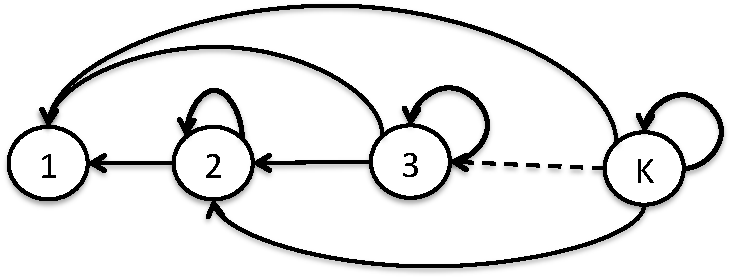
\includegraphics[scale=.5]{SideInfoGraph.pdf}
	\caption{Side observation graph $G^S$}
	\label{fig:SideObservationGraph]}
\end{wrapfigure} 
Further, any information provided by action $k>2$ is contained in that provided by all actions $k^\prime\geq k$-- if action $k$ is played in round $t$, then we observe predictions $\{\hat{Y}_t^1, \hat{Y}_t^2, \cdots, \hat{Y}_t^i\}$ which includes the observed predictions of all actions $k^\prime\leq i$. 
This side-observation can be represented by a directed graph $G^S=(V,E)$, where $|V|=K$ and $E=\{(i,j): i 1<i\leq j\leq K \}$. Note that $G^S$ has self loops for all nodes except for node $1$. The nodes in $G^S$ represents actions of the SAP and an edge $(i,j)\in E$ implies that actions $i$ provides information about action $j$. The side-observation graph for the SAP is shown in Figure (\ref{fig:SideObservationGraph]}).


\begin{thm}
	\label{thm:K-SAPRegret}
Let the dominance condition (\ref{eqn:DominanceCondition}) holds. Then SAP $\psi$ with $K\geq 2$ is regret equivalent to a MAB with side-observation graph $G^S$. 
\end{thm}

\begin{remark}
Note that the some of mean 	values $\{\gamma_1- \gamma_i - \sum_{j\leq i} c_j\}$ need not be positive. Since the stochastic bandit algorithms assume that reward lie in the interval $[0,1]$,  we can ensure positive means by setting distribution $\nu_k$, to have mean $\gamma_1- \gamma_i - \sum_{j< i} c_j + \sum_{k \leq K-1 }c_k$. Note that mean of each arm is shifted by the same amount, which does not change the regret value. This recovers the SAP with $K=2$ actions and Theorem \ref{thm:2SAPRegret} holds.
\end{remark}



\begin{proposition}[SAP regret lower bound]
	Let $\pi$ be any policy on SAT with 2 sensors such that it pulls the suboptimal arm only sub polynomial many times, i.e., $\mathbb{E}[N^\psi_i(T)]=o(T^a)$ for all $a>0$ and $i\neq i^*$. Then,
	\begin{equation}
	\liminf_{T \rightarrow \infty} R^\psi_T(\pi)/\log T \geq \kappa \mbox{	where  }
	\end{equation}
		\begin{align}
	\kappa=&\displaystyle\min_{\{w_i\}}\sum_{i \in [K]}(\mu_{i^*}- \mu_i) w_i \nonumber\\
	& \mbox{subjected to} \sum_{j i}w_i\geq 1/D(\mu_i + \sum_{j<i} c_j || \mu_{i^*}) \mbox{  for all } i\in [K]\\
	& w_i \geq 0 \mbox{ for all } i \in [K] \nonumber
	\end{align}
\end{proposition}

\begin{proposition}[K-SAT regret upper bound]
	Let $\pi^\prime$ denote a policy on a $K$-armed stochastic bandit where mean of arm $i>1$ is $\gamma_1-\gamma_i-\sum_{j<i}c_j$ and arm $1$ has a fixed reward of value zero, and the side-observation graph is $G^S$.  Then, the regret of a policy $g_1(\pi)$ for the SAT problem obtained from mapping (\ref{eqn:KBanditToSAP}) is upper bounded as
	\begin{equation}
	R^\psi_T(g(\pi))\leq \mathcal{O}(\xi(G^S)\log T + K^2)
	\end{equation}
	when $\pi^\prime=UCB-LP$ \cite{Sigmetrics15_StochasticBanditsWithSideObservations_BuccapatnamEriyilmazShroff}.
\end{proposition}




%
%\section{Extension to Multi-Stage and Multi-Action setting}
% 
% \subsection{Information and Side Observations:}
% on the feedback observed, we continue to assume that the dominance condition holds across the stages, i.e., for all $1\leq i\leq K-1$
% \begin{equation}
% \label{eqn:DominanceMultiStage}
%\mbox{ if } \hat{Y}_t^i=Y_t  \implies  \hat{Y}_t^j=Y_t \mbox{ for all } i<j\leq K
% \end{equation}
% Then, each time action $i>1$ is played, we get the same type of information about the loss incurred by an action pair  $(j,j-1)$ as in the SAP problem using the pair  $\{\hat{Y}_t^j,\hat{Y}_t^{j-1}\}$ for each $1<j<i$. Thus, playing action $i>1$ provides side observations about all the actions $j\leq ii$. We refer to this setting as Multi stage Sensor Acquisition Problem (MSAP). 
% 
% The side-observation structure in the MSAP problem can be represented by a directed graph $G=(\mathcal{V}, \mathcal{E})$ where $|\mathcal{V}|=K$ and $\mathcal{E}=\{(i,j) \in \mathcal{V}\times \mathcal{V}: i\geq j, i>1\}$. Here,  $(i,j)\in \mathcal{E}$ implies that selecting $i$ provides information about the prediction loss of action $j$. The side-observation graphs is depicted in Figure (\ref{fig:SideObservationGraph]}). Note that an edge $(i,j) \in \mathcal{E}$ only implies that playing action $i$ provides some information about the losses of actions $i\leq j$, but not their true losses. In the following we establish that regret of MSAP is equivalent to a stochastic $K$-armed bandit with the same side-observation structure.
%  \subsection{Regret Equivalence}
% \begin{thm}
% 	A MSAP $(K, \mathcal{A}, (\gamma_i,c_i)_{i\in [K]}, (L(i), F(i))_{i \in \mathcal{A}} )$ with $K>2$ is regret-equivalent to a stochastic bandit problem $(N, (\nu_i)_{i \in [N]})$ with $N=K$ and side observation structure give by $G$.
% \end{thm}	
%Consider a $K$-armed stochastic bandit problem where  reward distribution $\nu_k$ has mean $\gamma_1-\gamma_k + \sum_{j=2}^k c_j$ for all $1\leq k\leq K$, and the side-observation from arms is given by graphs $G$ . Given an arbitrary policy $\pi$ for the MSAP  that uses the side-information, we obtain a  policy BanditG($\pi$) for the bandit problem as follows: if BanditG($\pi$) played arm $i\neq 1$ in the previous round, it inputs the feedback observed from all arms $i\leq j$ to $\pi$ and copies $\pi$'s choice for next action. If BanditG($\pi$)  played arm $1$ in the previous round, it simply copies $\pi$'s choice for next action. Conversely, suppose $\theta$ is an arbitrary policy for the bandit problem with side-observation structure $G$, let MSAP($\theta$) denote a policy for MSAP that consults $\theta$ as follows: if MSAP($\theta$) played action $i$ in the previous round it inputs feedback vector $(0, \boldsymbol{1}_{\{\hat{Y}_t^j\neq \hat{Y}_t^{j-1} \}}, \forall \; j\leq 1)$ to $\theta$ and copies its choice for next action. Otherwise it simply copies $\theta$'s choice for next action.
%
%We next show that regret of BanditG($\pi$) on the bandit problem is same as that of $\pi$ on MSAP, 
% and regret of MSAP($\theta$) on MSAP is same as regret of $\theta$ on the bandit problem. 
% 
%For any strategy $\pi$, the expected regret of the MSAP can be expressed as 
%\begin{eqnarray}
%R_T(\pi) &=&\sum_{i=1}^{K}\left [ \left (\gamma_{i}+\sum_{j\leq i} c_j\right )-\left (\gamma_{i^*}+\sum_{j\leq i^*} c_j\right )\right ]\mathbb{E}[N_i(T)]\\
%&=&\sum_{i=1}^{K} \left[\left (\gamma_1+c_1-\gamma_{i^*}-\sum_{j\leq i^*} c_j \right )-\left (\gamma_1+c_1- \gamma_{i}-\sum_{j\leq i} c_j \right )\right ]\mathbb{E}[N_i(T)]
%\end{eqnarray} 
%where we added and subtracted $\gamma_1+c_1$ from each term. Now, notice that this is the expected regret of the policy on a stochastic bandit where the mean rewards  are 
%\begin{equation}
%\gamma_1+c_1 - \gamma_i - \sum_{j\leq i} c_j \quad \mbox{for } i=1,2,\cdots, K. 
%\end{equation}
%\begin{remark}
%Note that the some of mean 	values $\gamma_1+c_1 - \gamma_i - \sum_{j\leq i} c_j$ need not be positive. Since most of the stochastic bandit algorithms assume that reward lie in the interval $[0,1]$, they may not be directly applicable to our setting. However, this can be over come by setting the distributions of arm $k$, $\nu_k$, to have mean $\gamma_1+c_1 - \gamma_i - \sum_{j\leq i} c_j + \sum_{k=2}^K c_k$. Note that we translated the mean of each arm by the same amount this does not change the regret value. For $k=2$, this recovers the SAT problem and Theorem \ref{thm:SATRegret} holds
%\end{remark}
%$\wedge$
%
%\begin{thm}[Upper Bound]
%	
%\end{thm}
%\begin{thm}
%	
%\end{thm}
%When we pull an arm  $i$, we observe a realization of a distribution with mean $\gamma_1 -\gamma_i$, but since the cost values are fixed, this is equivalent to observe realization of a distribution with mean $\gamma_1 +c_1-\gamma_i + \sum_{j\leq i}c_i$. Thus, the sensor selection problem with mean costs $\{\gamma_i + \sum_{j\leq i}c_i\}$ is equivalent to a stochastic multi-armed problem with mean rewards $\{\gamma_1+c_1 -\gamma_i - \sum_{j\leq i}c_i\}$. 

% \alglanguage{pseudocode}
% \begin{algorithm}[!h]
% 	\footnotesize
% 	\caption{StAT-K}
% 	\label{Algorithm:Stochastic Apple Tasting1}
% 	\begin{algorithmic}[1]
% 		\State \textbf{Input:}
% 		\State $c_k$ cost of sensor $k=2\cdots,K $
% 		\State \textbf{Initialization:}
% 		\State Play $a_K$ once, observe $X_{j,t}^i$, for all $K \geq j>i\geq 1$
% 		\State $N_{K}(1)\leftarrow 1 $, $Y_{j,1}^i\leftarrow X_{j,1}^i$ and $\hat{\mu}_{j,1}^i\leftarrow \frac{Y_{j,1}^i}{N_{K}(1)}$ for all $K \geq j > i\geq 1$
% 		\For {$t = 2,3\cdots$}
% 		\State {\bf Select the best action optimistically. How? We can use pairwise information to select the best action as follows}  
% 		\For {$j=2,3,\cdots, K$}
% 		\State $I\leftarrow 1$
% 		\If {$\hat{\mu}_{j,t-1}^I + \sqrt{\frac{6\log t}{\sum_{k\geq j} N_{k}(t-1)}} > \displaystyle \sum_{k=I+1}^{j}c_k$}  \quad //Checks if action $I$ is better than action $i$,
% 		\State $I\leftarrow j$
% 		\Else
% 		\State $I \leftarrow I$
% 		\EndIf
% 		\EndFor
% 			\State play action $a_I$ and observe $X_{I,t}^i$ for all $I>i\geq 1$,
% 			\State $N_{I}(t) \leftarrow N_{I}(t-1)+1$, $Y_{I,t}^i\leftarrow Y_{I,t-1}^j+X_{I,t}^i$ for all $ I>i \geq 1$
% 			\State $\hat{\mu}_{I,t}^i \leftarrow \frac{Y_{I,t}^i}{\sum_{k=I}^{K}N_k(t)}$ for all $ I>i \geq 1$
% 		\EndFor 
% 		
% 		\Statex
% 	\end{algorithmic}
% 	% \vspace{-0.4cm}%
% \end{algorithm}
% 
%
%\section{Algorithm}
%Let $X_{j,t}^i=\boldsymbol{1}_{\{\hat{y}^{i}_t \neq \hat{y}^j_t\}}, j>i$ denote whether the predictions of sensors $i$ and $j$ agree or not in round $t$. Note that $X_{j,t}^i$ is observed whenever learner selects action $a_k, k>j$. Let $\hat{\mu}_{j,t}^i$ denote the empirical mean of the samples $\{X_{j,t}^t\}$ observed till time $s$, given by
%\begin{equation}
%\hat{\mu}_{j,s}^i= \frac{\sum_{t=1}^s X_{j,t}^i\boldsymbol{1}_{\{I_t\geq j\}}}{\sum_{k=j}^{K}N_k(s)}.
%\end{equation}
%
%
%{\bf Remarks: We discussed the strategy in Algorithm-1 (StAT-K). Consider the case of perfect knowledge of $\gamma_i$'s and assume $j^{th}$ action is optimal. Then we know that $\gamma_i - \gamma_j> \sum_{k=i+1}^{j} c_k$ for all $i<j$ and $\gamma_j - \gamma_i < \sum_{k=j+1}^{i} c_k$ for $j<i$. However, after estimating the $\gamma_i$'s and selecting the best action optimistically as in StAT-K does not lead to similar argument, i.e.,  suppose in round $t$, $I^{th}$ action is selected by StAT-K, then the following need not hold.}
%
%\[{\hat{\mu}_{I,t-1}^j + \sqrt{\frac{6\log t}{\sum_{k\geq I} N_{k}(t-1)}} > \displaystyle \sum_{k=j}^{I}c_k} \quad for \;\;  I>j\]
%and
%
%\[{\hat{\mu}_{j,t-1}^I + \sqrt{\frac{6\log t}{\sum_{k\geq j} N_{k}(t-1)}} < \displaystyle \sum_{k=I+1}^{j}c_k} \quad for \;\; j> I\]
%

\section{Extension to context based prediction}
\label{sec:Contextual}
In this section we consider that the prediction errors depend on the context $X_t$, and in each round the learner can decide which action to apply based on $X_t$. Let  $\gamma_i(X_t)=\Pr\{\hat{Y}^1_t \neq \hat{Y}^2_t| X_t\}$ for all $i \in [K]$. We refer to this setting as  Contextual Sensor Acquisition Problem (CSAP) and denote it as $\psi_c=(K, \mathcal{A}, \mathcal{C}, (\gamma_i,c_i)_{i\in [K]})$. 

Given $x \in \mathcal{C}$, let $L_t(a|x)$ denote the loss from action $a\in \mathcal{A}$ in round $t$. A policy on $\phi^c$ maps past history and current contextual information to an action. Let $\Pi^{\psi_c}$ denote set of policies on $\psi_c$ and for any policy $\pi \in \Pi^{\psi_c}$, let $\pi(x_t)$ denote the action selected when the context is $x_t$. For any sequence $\{x_t,y_t\}_{t>0}$, the regret of a policy $\pi$ is defined as:
\begin{equation}
R^{\phi_c}_T(\pi)= \sum_{t=1}^{T} \mathbb{E}\left [L_t(\pi(x_t)|x_t)\right ]-\sum_{t=1}^{T}\min_{a \in \mathcal{A}} \mathbb{E} \left [ L_t(a|x_t)\right ]. 
\end{equation}
As earlier, the goal is to learn a policy that minimizes the expected regret, i.e., $\pi^*= \arg \min_{\pi \in \Pi^{\psi_c}} \mathbb{E}[R^{\psi_c}_T(\pi)].$

In this section we focus on CSA-problem with two sensors and assume that sensor predictions errors are linear in the context. Specifically, we assume that there exists $\theta_1, \theta_2 \in \mathcal{R}^d$ such that $\gamma_1(x)=x^\prime\theta_1$ and $\gamma_2(x)+c=x^\prime\theta_2$ for all $x \in \mathcal{C}$, were $x^\prime$ denotes the transpose of $x$. By default all vectors are column vectors. In the following we establish that CSAP is regret equivalent to a stochastic liner bandits with varying decision sets. We first recall the stochastic linear bandit setup and relevant results. 

\noindent
{\bf Note: $c$ is a fixed cost and does not depend on context. We are assuming that error rate of sensor $2$ offset by $c$ is a linear quantity. Another possibility is, we can assume that there exists a $x_0 \in \mathcal{C}$ such that $c=x_0^\prime \theta_2 $ and we have oracle access to $x_0$. Then all the arguments hold.} 

\section{Background on Stochastic Linear Bandits}
In round $t$, the learner is given a decision set $D_t \subset \mathcal{R}^d$ from which he has to choose an action. For a choice $x_t \in D_t$, the learner receives a reward $r_t=x_t^\prime\theta^* + \epsilon_t$, where $\theta^* \in \mathcal{R}^d$ is unknown and $\epsilon_t$ is random noise of zero mean. The learner's goal  is to maximize the expected accumulated reward $\mathbb{E}\left[\sum_{t=1}^{T} r_t \right]$ over a period $T$. If the leaner knows $\theta^*$, his optimal strategy is to select $x_t^*=\arg \max_{x \in D_t} x^\prime \theta^* $ in round $t$. The performance of any policy $\pi$ that selects action $x_t$ at time $t$ is 
measured with respect to the optimal policy and is given by the expected regret  as follows
\begin{equation}
\label{eqn:LinearBanditRegret}
R^L_T(\pi)= \sum (x_t^*)^\prime \theta^* - \sum x_t^\prime \theta^* .
\end{equation}
The above setting, where actions sets can change in every round, is introduced in\cite{NIPS2011_ImprovedAlgorithms_AbbasiPalSzepes} and is a more general setting than that studied in \cite{COLT08_StochasticLinearOptimization_DaniHayesKakad,MOR11_LinearlyParametrized_RusmevichientongTsitsiklis} where decision set is fixed. Further, the above setting also specializes the contextual bandit studied in \cite{WWW10_Contextaulbandits_LiChuWei}. The authors in \cite{NIPS2011_ImprovedAlgorithms_AbbasiPalSzepes} developed an
`optimism in the face of uncertainty linear bandit algorithm' (OFUL) that achieves $\mathcal{O}(d \sqrt{T})$ regret with high probability when the random noise is $R$-sub-Gaussian for some finite $R$. The performance of OFUL is significantly better than $ConfidenceBall_2$ \cite{COLT08_StochasticLinearOptimization_DaniHayesKakad}, $UncertainityEllipsoid$ \cite{MOR11_LinearlyParametrized_RusmevichientongTsitsiklis}
and $LinUCB$ \cite{WWW10_Contextaulbandits_LiChuWei}. 


\begin{thm}
\label{thm:2CSAPRegret}
Consider a CSA-problem with $K=2$ sensors. Let $\mathcal{C}$ be a bounded set and $\gamma_i(x)+c_i=x^\prime\theta_i$ for $i=1,2$ for all $x \in \mathcal{C}$. Assume $x^\prime \theta_1, x^\prime \theta_2 \in [0\; 1]$ for all $x \in \mathcal{C}$. Then, equivalent to a stochastic linear bandit. 
\end{thm}



\newpage
\bibliographystyle{biblio}
%\bibliographystyle{IEEEtran}
\bibliography{bandits1}
\newpage
\appendix
\section{Proof of Theorem \ref{thm:2SAPRegret}}
Consider a $1$-armed stochastic bandit problem where arm with constant reward has value $c$ and the arm that gives stochastic reward has mean value  $\gamma_1-\gamma_2$.  
Given an arbitrary policy $\pi=(\pi_1, \pi_2, \cdots \pi_t )$ for the SAP, we obtain a policy for the bandit problem from $\pi$ as follows: Let $H_{t-1}$ denote the history, consisting of all arms played and the corresponding rewards, available to policy $\pi_{t-1}$ till time $t-2$. Let $a_{t-1}$ denote the action selected by the bandit policy  in round $t-1$ and $r_{t-1}$ the observed reward. Then, the next action $a_t$ is obtained as follows:
\begin{equation}
\label{eqn:SAPto1Bandit}
a_t=
\begin{cases}
\pi_t(H_{t-1}\cup \{1, \emptyset
\}) \mbox{ if } a_{t-1}= \mbox{fixed rewad arm}	\\
\pi_t(H_{t-1} \cup \{2, r_{t-1}\}) \mbox{ if } a_{t-1}= \mbox{stochastic arm}
\end{cases}
\end{equation}
\noindent
Conversely, let $\pi^\prime=\{\pi^\prime_1, \pi^\prime_2,\cdots\}$ denote an arbitrary policy for the 1-armed bandit problem. we obtain a policy for the SAP as follows: Let $H^\prime_{t-1}$ denote the history, consisting of all actions played and feedback, available to policy $\pi^\prime_{t-1}$ till time $t-1$. Let $a^\prime_{t-1}$ denote the action selected by the SAP policy in round $t-1$ and observed feedback $F_t$. Then, the next action $a^\prime_t$ is obtained as follows:
\begin{equation}
\label{eqn:1BanditToSAP}
a^\prime_t=
\begin{cases}
\pi^\prime_t(H^\prime_{t-1} \cup \{1, c
\}) \mbox{ if } a^\prime_{t-1}= \mbox{action 1}	\\
\pi^\prime_t(H^\prime_{t-1} \cup \{2, \boldsymbol{1}\{\hat{Y}_t^1\neq \hat{Y}_t^2\}\}) \mbox{ if } a_{t-1}= \mbox{actions 2}.
\end{cases}
\end{equation}
We next show that regret of $\pi$ on the SAP is same as that of derived policy on the 1-armed bandit, and  regret of $\pi^\prime$ on the 1-armed bandit is same as regret of the derived policy on SAP. 
We first argue that any policy on the SAP problem with 2 actions needs the information if whether the predictions of sensors match or not whenever action $2$ is played.  The following observation is straightforward.
\begin{lemma}
	\label{lma:SuffStat2Action}
	Let  dominance condition holds. Then, $\Pr\{\hat{Y}^1_t \neq \hat{Y}^2_t\}=\gamma_1-\gamma_2$.
\end{lemma}
\begin{eqnarray}
\lefteqn{\Pr\{\hat{Y}^1_t \neq \hat{Y}^1_t\}=\Pr\{\hat{Y}^1_t=Y_t, \hat{Y}^2_t \neq Y_t\} + \Pr\{\hat{Y}^2_t=Y_t, \hat{Y}^1_t \neq Y_t\}} \\
&=& \Pr\{\hat{Y}^2_t=Y_t, \hat{Y}^1_t \neq Y_t\} \;\;\mbox{from assumption (\ref{eqn:DominanceCondition})}\\
&=& \Pr\{\hat{Y}^1_t\neq y_t\}\Pr\{\hat{Y}^2_t= Y_t| \hat{Y}^1_t\neq Y_t\} \\
&=& \Pr\{\hat{Y}^1_t\neq Y_t\}\left( 1-\Pr\{\hat{Y}^2_t \neq  Y_t| \hat{Y}^1_t\neq Y_t\} \right ) \\
&=& \Pr\{\hat{Y}^1_t\neq Y_t\}\left( 1-\frac{\Pr\{\hat{Y}^2_t \neq  Y_t, \hat{Y}^1_t\neq Y_t\}}{\Pr\{\hat{Y}^1_t\neq Y_t\}} \right )\\
&=& \Pr\{\hat{Y}^1_t\neq Y_t\}-\Pr\{\hat{Y}^2_t \neq  Y_t\}  \;\; \mbox{by contrapositve of  (\ref{eqn:DominanceCondition})} 
\end{eqnarray}
From Lemma \ref{lma:SuffStat2Action}, mean of the observations $Z_t:=\boldsymbol{1}{\{\hat{Y}_t^1 \neq \hat{Y}_t^2 \}}$ from action $2$ in the SAP is a sufficient statistics to identify the optimal arm. Thus, any SAP only needs to know $Z_t$ in each round, and $Z_t$ are i.i.d with mean $\gamma_1-\gamma_2$.  Our mapping of policies is such that any poilcy for SAP (1-armed bandits) and the derived policy on the 1-armed bandit (SAP) play the sub-optimal arm same number of times.  For the sake of simplicity assume that action $1$ is optimal for SAP  $(\gamma_1> \gamma_2 + c)$ and let a policy $\pi$ on SAP plays it $N_1(T)$ number if times. Then, we have
\[ R^\psi_T(\pi)=\Delta_i\mathbb{E}[N^\psi_1(T)]=(\gamma_1-\gamma_2-c)\mathbb{E}[N_1(T)]\]
Let $f(\pi)$ denote the policy for the 1-armed bandit obtained using the mapping (\ref{eqn:SAPto1Bandit}). Now, for the $1$-armed bandit, where the arm with stochastic rewards is optimal, we have
\[ R^\phi_T(f(\pi))=(\mu_2-\mu_1)\mathbb{E}[N_1(T)]=(\gamma_1-\gamma_2-c)\mathbb{E}[N^\phi_1(T)]\]
Thus the regret of $\pi$ on the SAP problem and that of $f(\pi)$ on the $1$-armed bandit are the same. We can argue similarly for the other case. 


\section{Proof of Theorem \ref{thm:K-SAPRegret}}

Consider a $K$-armed stochastic bandit problem where rewards distribution $\nu_i$ has mean  $\gamma_1-\gamma_i- \sum_{j< i}c_j$ for all $i >1$ and arm $1$ gives a fixed reward of value $0$. The arms have side-observation structure defined by graph $G^S$.  
Given an arbitrary policy $\pi=(\pi_1, \pi_2, \cdots \pi_t )$ for the SAP, we obtain a policy for the bandit problem with side observation graph $G^S$ from $\pi$ as follows: Let $H_{t-1}$ denote the history, consisting of all arms played and the corresponding rewards, available to policy $\pi_{t-1}$ till time $t-2$. In round $t-1$, let $a_{t-1}$ denote the arm selected by the bandit policy,  $r_{t-1}$ the corresponding reward and $o_{t-1}$ the side-observation defined by graph $G_S$ excluding that from the first arm. Then, the next action $a_t$ is obtained as follows:
\begin{equation}
\label{eqn:SAPtoKBandit}
a_t=
\begin{cases}
\pi_t(H_{t-1}\cup \{1, \emptyset
\}) \mbox{ if } a_{t-1}= \mbox{arm 1}	\\
\pi_t(H_{t-1} \cup \{i, r_{t-1}\cup o_{t-1}\}) \mbox{ if } a_{t-1}= \mbox{arm i}
\end{cases}
\end{equation}
\noindent
Conversely, let $\pi^\prime=\{\pi^\prime_1, \pi^\prime_2,\cdots\}$ denote an arbitrary policy for the $K$-armed bandit problem with side-observation graph. we obtain a policy the SAP as follows: Let $H^\prime_{t-1}$ denote the history, consisting of all actions played and feedback, available to policy $\pi^\prime_{t-1}$ till time $t-2$. Let $a^\prime_{t-1}$ denote the action selected by the SAP policy in round $t-1$ and observed feedback $F_t$. Then, the next action $a^\prime_t$ is obtained as follows:
\begin{equation}
\label{eqn:KBanditToSAP}
a^\prime_t=
\begin{cases}
\pi^\prime_t(H^\prime_{t-1} \cup \{1, 0
\}) \mbox{ if } a^\prime_{t-1}= \mbox{action 1}	\\
\pi^\prime_t(H^\prime_{t-1} \cup \{i, \boldsymbol{1}\{\hat{Y}_t^1\neq \hat{Y}_t^2\}\cdots \boldsymbol{1}\{\hat{Y}_t^1\neq \hat{Y}_t^i\}\}) \mbox{ if } a_{t-1}= \mbox{action i}.
\end{cases}
\end{equation}
We next show that regret of a policy $\pi$ on the SAP problem is same as that of the policy derived from it for the $K$-armed bandit problem with side information graph $G^S$, 
and regret of $\pi^\prime$ on the $K$-armed bandit with side information graph  $G^S$ is same as that of the policy derived from it for the SAP.

Given a policy $\pi$ for the SAP problem let $f_1(\pi)$ denote the policy obtained by the mapping defined in (\ref{eqn:SAPtoKBandit}). The regret of policy $\pi$ that plays actions $i$, $N_i(T)$ times is given by 
\begin{eqnarray}
R^\psi_T(\pi) &=&\sum_{i=1}^{K}\left [ \left (\gamma_{i}+\sum_{j< i} c_j\right )-\left (\gamma_{i^*}+\sum_{j < i^*} c_j\right )\right ]\mathbb{E}[N^\psi_i(T)]\\
\end{eqnarray}
Now, regret of regret policy $f_1(\pi)$ on the $K$-armed bandit problem with side information graph $G^S$ 
\begin{equation}
R^{\phi_G}_T(f_1(\pi))=\sum_{i=1}^{K} \left[\left (\gamma_1-\gamma_{i^*}-\sum_{j <i^*} c_j \right )-\left (\gamma_1- \gamma_{i}-\sum_{j < i} c_j \right )\right ]\mathbb{E}[N^{\phi_G}_i(T)]
\end{equation}
which is same as $R^\phi_T(\pi)$. This concludes the proofs. 
\section{Proof of Theorem \ref{thm:2CSAPRegret}}
Let $\{x_t,y_t\}_{t\geq 0}$ be an arbitrary sequence of context-label pairs. Consider a stochastic linear bandit where $D_t=\{0, x_t\} $ is a decision set in round $t$. 
From the previous section, we know that given a context $x$, action $1$ is optimal if $\gamma_1(x)-\gamma_2(x) -c< 0$, otherwise  action $2$ is optimal. Let $\theta:=\theta_1-\theta_2$, then it boils down to check if $x^\prime\theta-c<0$ for each context $x\in \mathcal{C}$. 

For all $t$, define $\epsilon_t= \boldsymbol{1}\{\hat{Y}^1_t \neq \hat{Y}^2_t\}-x_t^\prime\theta$. Note that $\epsilon_t \in [0 \;1]$ for all $t$, and since sensors do not have memory, they are conditionally independent given past contexts. Thus, $\{\epsilon_t\}_{t>0}$ are conditionally $R$-sub-Gaussian for some finite $R$.  

Given a policy $\pi$ on a linear bandit we obtain next to play for the CSAP as follows: For each round $t$ define $a_t \in \mathcal{C}$ and $r_t \in \{0,1\}$ such that $a_t=0$ and $r_t=0$ if action $1$ is played in that round, otherwise set $a_t=x_t$ and $r_t=\boldsymbol{1}\{\hat{y}^1_t \neq \hat{y}^1_t \}$. Let $\mathcal{H}_{t}=\{(a_1, r_1)\cdots (a_{t-1},r_{t-1})\}$ denote the past actions and corresponding rewards observed till time $t-1$. In round $t$, after observing context $x_t$, we transfer  $((a_{t-1},r_{t-1}), D_t)$, where  $D_t=\{0,x_t\}$. If $\pi$ outputs $0 \in D_t$ as the optimal choice, we play action $1$, otherwise we play action $2$.

Conversely,   suppose $\pi^\prime$ denote a policy for the CSAP problem we select action to play from decision set $D_t=\{0,x_t\}$ as follows.  For each round $t$ define $a^\prime_t \in {1,2}$ and $r^\prime_t \in \mathcal{R}$ such that $a^\prime_t=1$ and $r^\prime_t=\emptyset$ if $0$ is played otherwise set $a^\prime_t=2$ and $r^\prime_t=x_t^\prime\theta^* +\epsilon_t$ if $x_t$ is played.  Let $\mathcal{H}^\prime_{t}=\{(a^\prime_1, r^\prime_1)\cdots (a^\prime_{t-1},r^\prime_{t-1})\}$ denote the past actions and corresponding rewards observed till time $t-1$. In round $t$, after observing set  $D_t$, we transfer  $((a^\prime_{t-1},r^\prime_{t-1}), x_t)$ to policy $\pi^\prime$. If $\pi$ outputs action $1$ as the optimal choice, we play action $0$, otherwise we play $x_t$. 

%\todoc{However, the crowdsourcing model is also unidentifiable in a strict sense; and the rank one assumption is what saves the day there.}
%\section{Calibrating the sensors}
%In this sections we assume that the predictions accuracy can be controlled. Let $\hat{\hat{y}}^i_t$ denote the measurement output by device-i in round $t$. The prediction of device-i is given by 
%\begin{equation}
%\hat{y}^i_t=\mbox{sign}(\hat{\hat{y}}^i_t-\eta_i)
%\end{equation}
%where $\eta_i \in \mathcal{R}$ is the calibration parameter set by the learner. Thus, setting $\eta_i$ the learner can control the prediction accuracy of the devices.  A policy involves selecting a device and setting its calibration parameter in each round. The goal is to learn a policy that minimizes the expected regret defined in \ref{eqn:Regret2Actions}.    

%\section{Relationship to crowdsourcing}
%A basic problem formulation in crowdsourcing is the following:%
%\footnote{
%	See
%	\url{https://uwspace.uwaterloo.ca/bitstream/handle/10012/9841/Szepesvari_David.pdf?sequence=1&isAllowed=y}
%	and the references therein.}
%One is given a $W \times T$ table $Y$ of binary labels (for convenience, $Y\in \{\pm \}^{W\times T}$), the $(w,t)$th entry $Y_{wt}$ in the table corresponding to the response of worker $w$ for task $t$. 
%It is assumed that the performance of each worker is stable across the tasks and that tasks are also randomly chosen from a fixed distribution. More precisely, $Y_{w,t} = (\xi_{w,t,-1} \one{ Y^*_t=-1} + \xi_{w,t,+1}  \one{ Y^*_t=+1}) Y^*_{t}$, where $Y^*_{t}\in \{\pm 1\}$ is the ``true'' unobserved label, $\xi_{w,t,y}\in \{\pm 1\}$ is the variable that indicates corruption of label $y\in \{\pm 1\}$ of worker $w$ in task $t$. It is assumed that $(Y^*_t)_{1\le t\le T}$, $(\xi_{w,t,y})_{w,t,y}$ are mutually independent of each other,
%while $Y^*_t \sim_D Y^*_{t'}$ and $\xi_{w,t,y} \sim_D \xi_{w,t',y}$ for any $t,t',w,y$.
%The joint distribution of the random variables in the observed table $Y$ is thus uniquely determined by the probabilities $\Prob{ Y^*_1 = +1 }$ and $\Prob{ \xi_{w,1,y} = +1 }$, $1\le w \le W$, $y\in \{\pm 1\}$. The model described dates back to the work of Dawid and Skene in 1979.\footnote{Dawid,  P.,  Skene,  A. M.,  Dawid,  A. P.,  and Skene,  A. M. (1979).  Maximum likelihood
%	estimation  of  observer  error-rates  using  the  EM  algorithm. Applied  Statistics,  pages 20--28.}
%
%One basic task in crowdsourcing is to infer the values of $(Y_t^*)_{1\le t\le T}$ given the observed table $Y$. This is called the inference problem (this is often studied even in the lack of assumptions on the task generation process). Very often, this is studied under the so-called symmetric noise assumption when $\xi_{w,t,y}$ and $\xi_{w,t,-y}$ are identically distributed. In this case, the optimal way to aggregate the labels provided by the workers is to use a weighted majority vote, i.e., using $\sgn( \sum_{w=1}^W v_w Y_{w,t} )$ to predict the label for task $t$, where $v_w^* = \ln( \frac{1+s_w^*}{1-s_w^*} )$ and $s_w^* = \Prob{\xi_{w,1,1}=1}-\Prob{\xi_{w,1,1}=-1}$ denotes the ``skillfulness'' of worker $w$.  In the lack of the knowledge of worker skill levels, the skills are estimated. This is based on writing $Y_{w,t} = \xi_{w,t} Y^*_t = s_w^* Y^*_t + Z_{w,t} Y_t^*$, where $\EE{Z_{w,t}|Y^*_t} = 0$ and we used that $\EE{ \xi_{w,t,1}|Y^*_t} = s_w^*$. Thus, $Y$ can be viewed as a noisy observation of a rank-one matrix.
%
%Note that in the lack of the symmetry assumption, the rank-one approximation becomes a rank-two approximation, a case, which, to the best of our knowledge, has not been studied theoretically in the literature so far.
%
%
%\section{Dependence of $\gamma_1$ and $\gamma_2$ on a Discrete Space of $x_t$}
%\subsection{Independence Across Symbols}
%Equivalent to playing multiple constant problems in parallel.
%\subsection{Smoothness Assumption}
%Assume $\|\gamma_1(x_1)-\gamma_1(x_2)\|\leq \beta \|x_1-x_2\|$ and $\|\gamma_2(x_1)-\gamma_2(x_2)\|\leq \beta \|x_1-x_2\|$ for all $x_1,x_2$. Now observations for a single value of $x_t$ are informative across the space of discrete $x$. How does this change the algorithm/performance? This should generalize to the continuous space of $x$.

\end{document} 
